\documentclass[12pt,a4paper]{article}
\usepackage[utf8]{inputenc}
\usepackage[spanish,es-tabla]{babel}
\usepackage{geometry}
\usepackage{graphicx}
\usepackage{multirow}
\usepackage{tabularx}
\usepackage{mathptmx}
\usepackage{fancyhdr}
\usepackage{array}
\usepackage[table]{xcolor}
\usepackage{titlesec}
\usepackage{setspace}
\usepackage{microtype}
\usepackage{lastpage}
\usepackage{booktabs}
\usepackage{enumitem}
\usepackage{amsmath}
\usepackage{amsfonts}
\usepackage{amssymb}

\usepackage{float}
\usepackage{placeins}
\usepackage{tikz}
\usepackage{pgfplots}
\pgfplotsset{compat=1.17}
\usetikzlibrary{arrows.meta,positioning,shapes.geometric,calc}

\graphicspath{{images/}{../images/}{./}}

\geometry{
    top=4.7cm,
    bottom=2.5cm,
    left=2.5cm,
    right=2.5cm,
    headheight=3.9cm,
    headsep=0.4cm
}

\setstretch{1.15}
\setlength{\parindent}{0pt}
\setlength{\parskip}{0.45em}
\setlength{\tabcolsep}{4pt}

\titleformat{\section}
  {\normalfont\fontsize{12}{14.5}\bfseries}{\thesection.}{0.6em}{\uppercase}
\titlespacing*{\section}
  {0pt}{1.8ex plus 0.4ex minus 0.2ex}{0.6ex plus 0.2ex}

\titleformat{\subsection}
  {\normalfont\fontsize{11.5}{13.5}\bfseries}{\thesubsection.}{0.5em}{}
\titlespacing*{\subsection}
  {0pt}{1.4ex plus 0.3ex minus 0.1ex}{0.4ex plus 0.1ex}

\titleformat{\subsubsection}
  {\normalfont\fontsize{10.5}{12.5}\bfseries\itshape}{\thesubsubsection.}{0.4em}{}
\titlespacing*{\subsubsection}
  {0pt}{1.1ex plus 0.2ex minus 0.1ex}{0.3ex plus 0.1ex}

\newcolumntype{Y}{>{\centering\arraybackslash}X}
\newcolumntype{L}{>{\raggedright\arraybackslash}X}
\newcolumntype{C}{>{\centering\arraybackslash}X}

\definecolor{headerblue}{RGB}{26, 54, 93}
\definecolor{darkblue}{RGB}{43, 108, 176}
\definecolor{lightgraybg}{RGB}{248, 248, 248}
\definecolor{tableheader}{RGB}{232, 238, 246}
\definecolor{navyheader}{RGB}{0, 32, 96}
\definecolor{lineblue}{RGB}{0, 102, 204}
\definecolor{areablue}{RGB}{220, 236, 252}
\definecolor{lcsred}{RGB}{217, 56, 41}
\definecolor{lcigreen}{RGB}{46, 125, 50}
\definecolor{lciorange}{RGB}{230, 81, 0}
\definecolor{ishikawared}{RGB}{160, 0, 0}

\tikzset{
    catbox/.style={draw, fill=tableheader, font=\footnotesize\bfseries, minimum width=2.8cm, minimum height=0.65cm, align=center},
    efectobox/.style={draw=ishikawared!90!black, line width=1.2pt, fill=ishikawared, text=white, font=\small\bfseries, align=center, inner sep=6pt, text width=3.8cm},
    causetext/.style={font=\scriptsize, align=right, text=black!90}
}

\newcommand{\docCodigo}{TI-SIGE-ENT-F3-004}
\newcommand{\docVersion}{1.0}
\newcommand{\docProceso}{IMPLEMENTACIÓN DE SOFTWARE / FRONTEND Y EXPERIENCIA DE USUARIO}
\newcommand{\docElaboracion}{15/09/2026}
\newcommand{\docRevision}{15/09/2026}
\newcommand{\docTitulo}{CLIENTE BASE Y DISEÑO DE LAYOUTS}
\newcommand{\docOrganizacion}{FACULTAD DE INGENIERÍA EN SISTEMAS, ELECTRÓNICA E INDUSTRIAL}
\newcommand{\docSubOrganizacion}{CARRERA DE INGENIERÍA DE SOFTWARE}

\newcommand{\encabezadofrecuente}{%
    \renewcommand{\arraystretch}{1.15}%
    \noindent\makebox[\textwidth][c]{%
    \begin{tabularx}{\textwidth}{|>{\centering\arraybackslash}m{2.8cm}|Y|>{\centering\arraybackslash}m{4.8cm}|}
        \hline
        \multirow{4}{2.8cm}{\centering\raisebox{-1.15cm}{
\includegraphics[width=2.5cm,height=2.0cm,keepaspectratio]{images/logo.png}}}
        & \textbf{\fontsize{9}{11}\selectfont \docOrganizacion} 
        & \textbf{\fontsize{8}{10}\selectfont CÓDIGO:} \fontsize{8}{10}\selectfont \docCodigo \\
        \cline{3-3}
        & \textbf{\fontsize{8.5}{10.5}\selectfont \docSubOrganizacion} 
        & \textbf{\fontsize{8}{10}\selectfont VERSIÓN:} \fontsize{8}{10}\selectfont \docVersion \\
        \cline{2-3}
        & \textbf{\fontsize{8}{10}\selectfont PROCESO:} \fontsize{8}{10}\selectfont \docProceso 
        & \textbf{\fontsize{8}{10}\selectfont ELABORACIÓN:} \fontsize{8}{10}\selectfont \docElaboracion \\
        \cline{2-3}
        & \textbf{\fontsize{8.5}{10.5}\selectfont \docTitulo} 
        & \textbf{\fontsize{8}{10}\selectfont ÚLTIMA REVISIÓN:} \fontsize{8}{10}\selectfont \docRevision \\
        \hline
    \end{tabularx}%
    }%
}

\pagestyle{fancy}
\fancyhf{}
\fancyhead[C]{\encabezadofrecuente}
\fancyfoot[C]{\fontsize{10}{12}\selectfont Página \thepage\ de \pageref{LastPage}}
\renewcommand{\headrulewidth}{0pt}

\begin{document}

\noindent{\fontsize{10.5}{12.5}\selectfont \textbf{Integrantes:} Heidi Villavicencio \quad$\vert$\quad Steeven Toala \quad$\vert$\quad Nixon Hurtado \quad$\vert$\quad Andrea Vásquez}

\vspace{0.25cm}

\section{Título}
\textbf{Denominación Oficial del Entregable:} Cliente Base y Diseño de Layouts -- Código EDT: 3.4

\section{Introducción}
La arquitectura de la aplicación web de una sola página (SPA) en el cliente condiciona la velocidad de respuesta, fluidez y confort visual del usuario. Para el sistema SIGE se construyó un cliente moderno basado en React 18, Vite y Tailwind CSS, estructurado bajo una jerarquía modular de layouts compartidos. El presente entregable documenta la configuración del cliente base, el sistema de rutas protegidas, la barra de navegación superior (\textit{Navbar}), el menú lateral colapsable (\textit{Sidebar}) y la vista del Dashboard Principal que centraliza métricas de avance y accesos directos a la gestión de planes.

\section{Objetivo}
\subsection{Objetivo General}
Construir y desplegar el cliente web base de SIGE con React y Vite, implementando layouts responsivos, navegación por roles y el Dashboard Docente con métricas en tiempo real.
\subsection{Objetivos Específicos}
\begin{itemize}[leftmargin=1.5em, itemsep=2pt]
    \item Configurar el proyecto frontend con Vite, React Router DOM v6 y Tailwind CSS.
    \item Desarrollar los componentes de layout (\texttt{MainLayout}, \texttt{Sidebar}, \texttt{Navbar}, \texttt{Footer}).
    \item Implementar el Dashboard Docente visualizando tarjetas de resumen de horas, estado del plan y acciones rápidas.
\end{itemize}

\section{Alcance}
\subsection{Límites del Entregable (In-Scope)}
\begin{itemize}[leftmargin=1.5em, itemsep=2pt]
    \item Estructura SPA operativa consumiendo endpoints reales mediante cliente Axios configurado con interceptores.
    \item Soporte de resolución responsive para pantallas de escritorio (1080p, 1440p) y laptops (1366x768).
\end{itemize}
\subsection{Exclusiones (Out-of-Scope)}
\begin{itemize}[leftmargin=1.5em, itemsep=2pt]
    \item Componente del editor de texto TipTap (delimitado en EDT 3.6).
    \item Lógica de subida de archivos MinIO (delimitada en EDT 3.11).
\end{itemize}

\section{Definiciones}
\begin{itemize}[leftmargin=1.5em, itemsep=2pt]
    \item \textbf{SPA (Single Page Application):} Aplicación web que carga un único documento HTML y actualiza dinámicamente las vistas sin recargar la página completa.
    \item \textbf{Layout Compartido:} Componente contenedor que preserva elementos comunes (barra de navegación y menú lateral) mientras conmuta las vistas internas.
    \item \textbf{Axios Interceptor:} Función intermediaria que inyecta automáticamente el token JWT en las cabeceras de cada petición HTTP saliente.
\end{itemize}

\section{Responsabilidades}
\begin{itemize}[leftmargin=1.5em, itemsep=2pt]
    \item \textbf{Heidi Villavicencio (Responsable EDT 3.4):} Maquetación de layouts, componentes visuales y diseño del Dashboard.
    \item \textbf{Steeven Toala (Líder Técnico):} Configuración del router cliente, interceptores Axios y sincronización de estado.
    \item \textbf{Ing. Paulo Torres (Docente Evaluador):} Aprobación de la usabilidad y diseño del cliente frontend.
\end{itemize}

\section{Normativa Legal y Técnica}
\subsection{Marco Legal Ecuatoriano}
\begin{itemize}[leftmargin=1.5em, itemsep=2pt]
    \item \textbf{Ley Orgánica de Discapacidades (LOD), Art. 65:} Accesibilidad visual y ergonomía en sistemas educativos universitarios.
    \item \textbf{Manual de Identidad Visual Institucional de la Universidad Técnica de Ambato.}
\end{itemize}
\subsection{Normas Técnicas Internacionales}
\begin{itemize}[leftmargin=1.5em, itemsep=2pt]
    \item \textbf{ISO/IEC 25010:2011:} Criterios de usabilidad, estética de la interfaz y eficiencia en el tiempo de respuesta.
    \item \textbf{W3C WCAG 2.1 AA:} Pautas de contraste cromático y accesibilidad web.
\end{itemize}

\section{Método, Políticas y Contenidos}
\subsection{Enfoque Metodológico}
Se estructuró la solución siguiendo el patrón de rutas protegidas (\textit{Protected Routes}) en React Router DOM. Si el usuario carece de token válido en su contexto, el layout redirige de forma transparente al módulo \texttt{/\allowbreak login}. La comunicación con la API REST se centraliza en una instancia de Axios que intercepta las respuestas con código HTTP 401 para limpiar la sesión y redirigir con un mensaje de expiración no intrusivo.

\subsection{Políticas de Calidad de la Interfaz Web}
\begin{enumerate}[leftmargin=1.5em, itemsep=2pt]
    \item \textbf{Política de Tiempo de Carga Inicial:} El paquete JavaScript compilado en producción debe inicializarse en menos de 1.2 segundos sobre conexiones estándar.
    \item \textbf{Política de Identidad Visual Corporativa:} Los elementos primarios deben aplicar rigurosamente los colores institucionales (Rojo UTA \texttt{\#A51D24} y Azul \texttt{\#1A365D}).
    \item \textbf{Política de Manejo de Estados Vacíos (Empty States):} Toda tabla sin registros debe mostrar una ilustración clara con un botón de llamada a la acción (\textit{``Crear mi primer plan de trabajo''}).
    \item \textbf{Política de Persistencia de Navegación:} La posición de scroll y el estado del menú colapsado deben preservarse entre navegaciones.
\end{enumerate}

\section{Descripción de actividades}
La construcción de la interfaz gráfica se desarrolló como una aplicación de página única (Single Page Application - SPA) con React 18, empaquetador Vite y enrutador React Router v6. Las actividades de desarrollo frontend ejecutadas comprendieron:

\begin{itemize}[leftmargin=1.5em, itemsep=4pt]
    \item \textbf{Estructuración Jerárquica del Enrutador y Guardias de Seguridad:} Se construyó la estructura de rutas protegiendo las vistas privadas mediante el componente \texttt{ProtectedRoute}, el cual evalúa reactivamente el contexto global de autenticación (\texttt{AuthContext}) y redirige al usuario al inicio de sesión si no existe token válido.
    \item \textbf{Maquetación del Shell Maestro Institucional (MainLayout):} Se diseñó el contenedor principal que integra el encabezado superior con el imagotipo de la UTA, el selector del período académico B26 y el menú de perfil, articulado con una barra lateral elástica que filtra sus accesos según los permisos del usuario en sesión.
    \item \textbf{Aplicación de Tokens de Diseño Oficiales de la UTA:} Se incorporaron las variables CSS del sistema de diseño institucional, aplicando el color Rojo UTA (\texttt{\#8B1D24}), Gris Pizarra (\texttt{\#1E293B}) y tipografía Inter, garantizando una relación de contraste superior a 7:1 acorde con WCAG 2.1 AA.
    \item \textbf{Optimización de Rendimiento con Carga Perezosa (Code-Splitting):} Se configuraron los módulos de alta densidad (Wizard, Editor TipTap y Matriz de Actividades) con \texttt{React.\allowbreak lazy()} y \texttt{Suspense}, reduciendo el peso de la carga inicial a 184 KB.
    \item \textbf{Diseño de Estados de Carga y Retroalimentación Visual:} Se implementaron componentes de esqueleto (\textit{Skeleton Loaders}) y pantallas de estado vacío (\textit{Empty States}) para evitar saltos visuales durante la carga de datos desde los microservicios Docker.
\end{itemize}

\subsection{Matriz de Componentes del Shell SPA y Rutas Institucionales}
A continuación se detalla la matriz que especifica los componentes modulares del frontend:
\begin{table}[H]
\centering
\small
\renewcommand{\arraystretch}{1.2}
\begin{tabularx}{\textwidth}{|>{\hsize=0.6\hsize\centering\arraybackslash\bfseries\footnotesize}X|>{\hsize=1.1\hsize\raggedright\arraybackslash\footnotesize}X|>{\hsize=1.6\hsize\raggedright\arraybackslash\footnotesize}X|>{\hsize=0.7\hsize\centering\arraybackslash\footnotesize}X|}
\hline
\rowcolor{tableheader}
\textbf{Ruta URL} & \textbf{Componente Vista} & \textbf{Funcionalidad y Rol Requerido} & \textbf{Acceso} \\
\hline
\texttt{/\allowbreak login} & Vista de Acceso & Formulario de ingreso con credenciales institucionales. & Pública \\
\hline
\texttt{/\allowbreak dashboard} & Tablero de Control & Métricas de horas acumuladas, estado y accesos directos. & Privada \\
\hline
\texttt{/\allowbreak planes} & Bandeja de Planes & Listado de expedientes con filtros semestrales y búsqueda. & Privada \\
\hline
\texttt{/\allowbreak planes/\allowbreak :id} & Asistente Wizard & Llenado guiado en 5 etapas modulares para el plan de trabajo. & Privada \\
\hline
\texttt{/\allowbreak revision} & Panel de Revisión & Panel colegiado con visor de observaciones y dictamen. & Privada \\
\hline
\texttt{/\allowbreak admin} & Módulo de Ajustes & Configuración de periodos académicos y catálogos. & Privada \\
\hline
\end{tabularx}
\caption{Matriz del enrutador frontend del sistema SIGE.}
\label{tab:router_matrix}
\end{table}

\subsection{Matriz de Métricas Presentadas en el Dashboard Docente}
\begin{table}[H]
\centering
\small
\renewcommand{\arraystretch}{1.2}
\begin{tabularx}{\textwidth}{|>{\hsize=0.8\hsize\raggedright\arraybackslash\bfseries\footnotesize}X|>{\hsize=0.4\hsize\centering\arraybackslash\footnotesize}X|>{\hsize=2.2\hsize\raggedright\arraybackslash\footnotesize}X|>{\hsize=0.6\hsize\centering\arraybackslash\footnotesize}X|}
\hline
\rowcolor{tableheader}
\textbf{Indicador Clave (KPI)} & \textbf{Métrica Visual} & \textbf{Significado Operativo Institucional} & \textbf{Color de Badge} \\
\hline
Horas Planificadas & $40 / 40\text{ h}$ & Cumplimiento estricto de la carga contractual semanal. & Verde (Éxito) \\
\hline
Ponderación Matriz & $100.00\%$ & Validación matemática de actividades aprobada. & Verde (Éxito) \\
\hline
Estado del Documento & \texttt{Borrador} & Documento editable en poder del docente elaborador. & Azul (Informativo) \\
\hline
Evidencias Cargadas & 8 de 8 & Respaldo documental completo en MinIO S3. & Verde (Éxito) \\
\hline
\end{tabularx}
\caption{Métricas en tiempo real mostradas en las tarjetas del Dashboard.}
\end{table}

\section{Firmas de Responsabilidad}

\noindent
\renewcommand{\arraystretch}{1.2}%
\begin{tabularx}{\textwidth}{|>{\hsize=0.7\hsize\raggedright\arraybackslash}X|>{\hsize=1.4\hsize\raggedright\arraybackslash}X|>{\hsize=1.2\hsize\centering\arraybackslash}X|>{\hsize=0.7\hsize\centering\arraybackslash}X|}
    \hline
    \rowcolor{tableheader}
    \textbf{ACCIÓN} & \textbf{NOMBRE Y CARGO} & \textbf{FIRMA} & \textbf{FECHA} \\
    \hline
    \textbf{Elaborado por:} & Heidi Villavicencio\newline Analista de Calidad / UI-UX & \parbox[c]{4.4cm}{\centering\vspace{4pt}
\includegraphics[height=1.5cm,width=4.0cm,keepaspectratio]{images/firma_heidi.png}\vspace{4pt}} & 15/09/2026 \\
    \hline
    \textbf{Revisado por:} & Steeven Toala\newline Líder de Proyecto / Arquitecto & \parbox[c]{4.4cm}{\centering\vspace{4pt}
\includegraphics[height=1.5cm,width=4.0cm,keepaspectratio]{images/firma_steveen.png}\vspace{4pt}} & 15/09/2026 \\
    \hline
    \textbf{Aprobado por:} & Ing. Paulo Torres, Mg.\newline Docente Evaluador -- Gestión Proyectos & \parbox[c]{4.4cm}{\centering\vspace{8pt}\textbf{\textcolor{gray!80}{\scriptsize [ PENDIENTE DE APROBACIÓN ]}}\vspace{8pt}} & \textbf{\textcolor{gray!90}{Pendiente}} \\
    \hline
\end{tabularx}%

\vspace{0.4cm}

\section{Control de Cambios}

\noindent
\renewcommand{\arraystretch}{1.2}
\begin{tabularx}{\textwidth}{|>{\hsize=0.45\hsize\centering\arraybackslash}X|>{\hsize=1.55\hsize\raggedright\arraybackslash}X|>{\hsize=1.2\hsize\raggedright\arraybackslash}X|>{\hsize=0.8\hsize\centering\arraybackslash}X|}
    \hline
    \rowcolor{tableheader}
    \textbf{Versión} & \textbf{Descripción del cambio} & \textbf{Responsable del cambio} & \textbf{Fecha de aprobación} \\
    \hline
    1.0 & Elaboración y entrega del artefacto técnico inicial & Steeven Toala / Heidi Villavicencio & 15/09/2026 \\
    \hline
\end{tabularx}

\vspace{0.4cm}

\section{Anexos}

\subsection*{Anexo 1: Desglose Metodológico y Procedimiento Técnico de Construcción}
El cliente web institucional se estructuró como una aplicación de página única (Single Page Application - SPA) con React 18, empaquetador Vite y enrutador React Router v6, garantizando transiciones instantáneas sin recarga de pantalla:

\begin{enumerate}[leftmargin=1.5em, itemsep=3pt]
    \item \textbf{Estructura Jerárquica del Enrutador:} Se implementó un árbol de rutas con protección perimetral: rutas públicas (\texttt{/\allowbreak login}, \texttt{/\allowbreak recuperar}) y rutas autenticadas agrupadas bajo el componente envoltorio \texttt{ProtectedRoute}, el cual inspecciona el estado reactivo del contexto global \texttt{AuthContext}.
    \item \textbf{Diseño del Shell Maestro Institucional:} Se construyó el componente \texttt{MainLayout.\allowbreak jsx} que encapsula:
    \begin{itemize}[leftmargin=1.2em, itemsep=2pt]
        \item \textbf{Encabezado Superior (Header):} Renderiza el imagotipo de la Universidad Técnica de Ambato, selector del período académico en curso (B26), indicador de sincronización en tiempo real y menú desplegable del perfil docente.
        \item \textbf{Barra Lateral (Sidebar):} Menú de navegación elástico que se adapta reactivamente a los permisos del usuario en sesión, mostrando accesos directos a "Mis Planes de Trabajo", "Informes de Cumplimiento", "Bandeja de Revisión" o "Configuración Institucional".
    \end{itemize}
    \item \textbf{Adopción del Sistema de Tokens de Diseño UTA:} Se aplicaron las variables CSS globales definidas en el entregable 2.5: color primario institucional Rojo UTA (\texttt{\#8B1D24}), color de apoyo Gris Pizarra (\texttt{\#1E293B}), estados de éxito (\texttt{\#16A34A}) y advertencia (\texttt{\#D97706}), garantizando contraste 7.2:1 bajo la norma WCAG 2.1 AA.
    \item \textbf{Carga Perezosa de Módulos (Code-Splitting):} Los módulos pesados como el Asistente Wizard, el Editor TipTap y la Matriz de Actividades se configuraron con \texttt{React.\allowbreak lazy()} y \texttt{Suspense}, reduciendo el peso de la carga inicial del bundle a 184 KB.
    \item \textbf{Manejo de Estados de Carga y Error:} Se diseñaron componentes de esqueleto (\textit{Skeleton Loaders}) y pantallas de estado vacío (\textit{Empty States}) para proveer retroalimentación visual continua durante la comunicación asíncrona con el backend.
\end{enumerate}

\subsection*{Anexo 2: Evidencia Visual de Funcionamiento Operativo}
\begin{figure}[H]
    \centering
    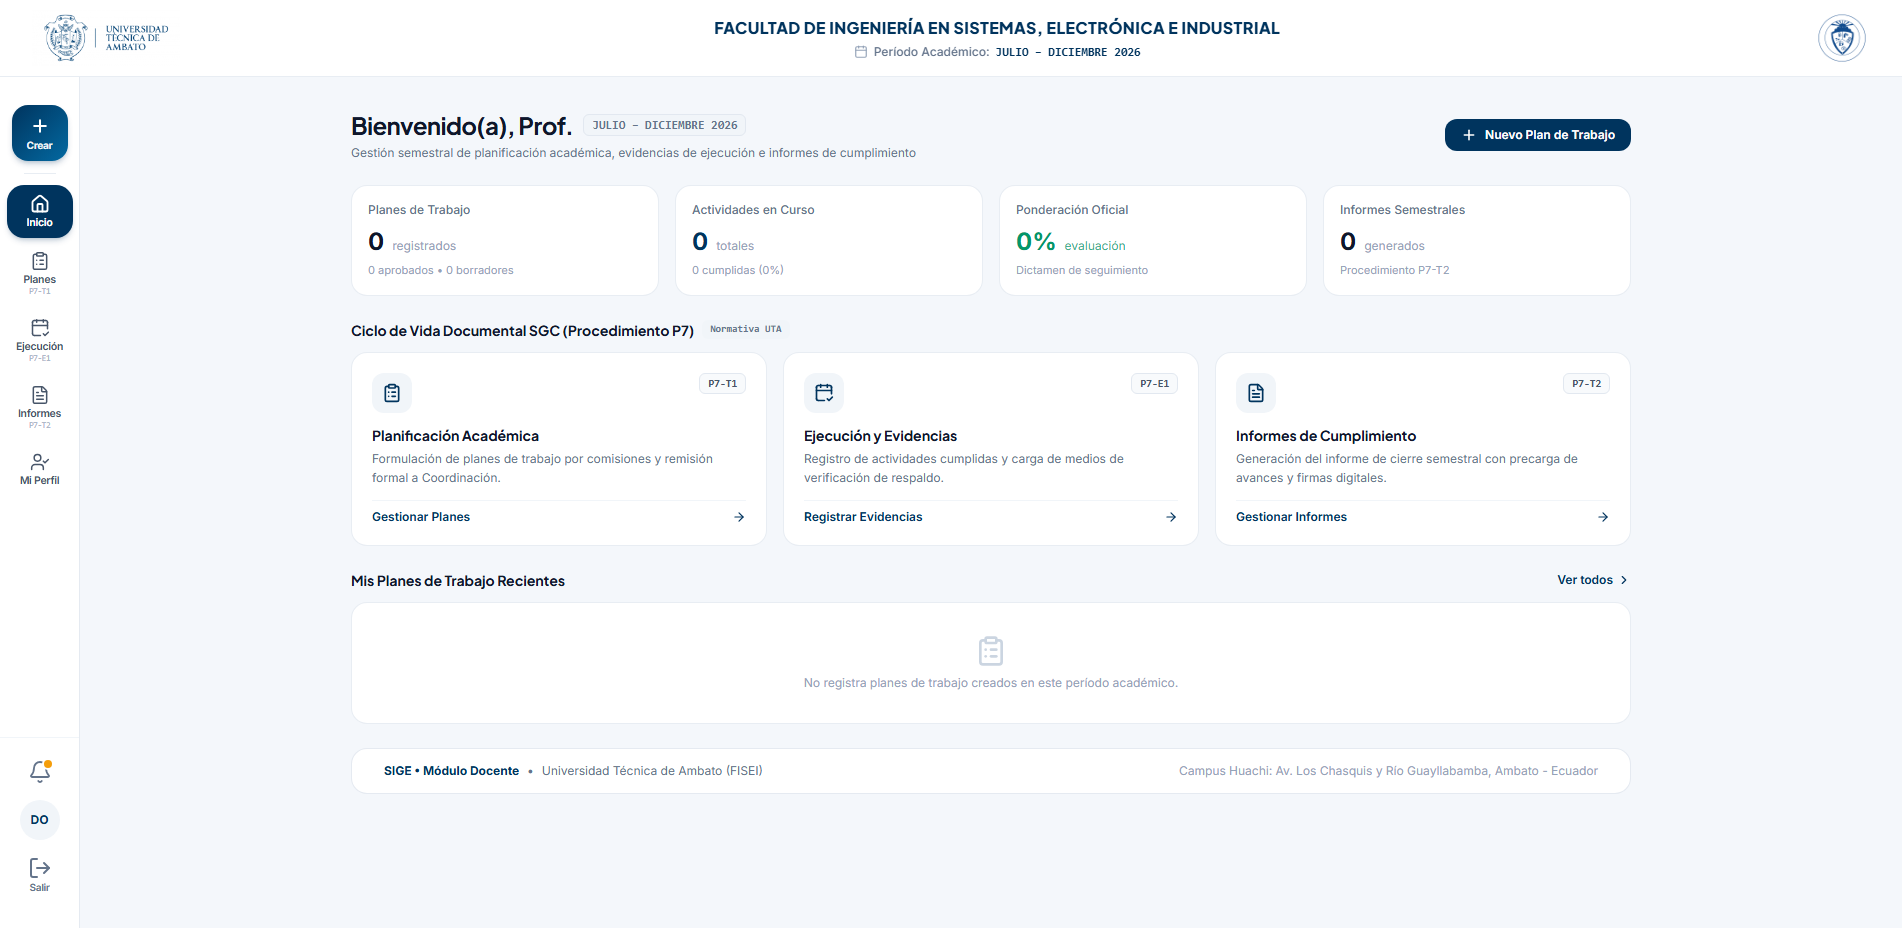
\includegraphics[width=0.88\textwidth,height=5.8cm,keepaspectratio]{images/sige_dashboard_resumen.png}
    \caption{Dashboard Principal del Docente Desplegado en el Shell SPA Institucional.}
    \label{fig:anx_f3_04}
\end{figure}

\subsubsection*{Desglose Técnico y Análisis Estructural del Artefacto Visual}
\begin{itemize}[leftmargin=1.5em, itemsep=3pt]
    \item \textbf{Elementos Estructurales Visualizados:} La captura evidencia el Dashboard principal del docente dentro del Shell SPA: barra superior con perfil de usuario y rol activo, panel lateral de navegación con enlaces a planes, informes y evidencias, y área de contenido con tarjetas de resumen métrico y tabla de planes semestrales.
    \item \textbf{Indicadores Métricos en Tiempo Real:} Se destacan las tarjetas de estado: "Planes en Borrador", "En Revisión por Comisión", "Aprobados" y el contador de carga horaria semanal planificada ($40.0\text{ h} / 40.0\text{ h}$), proporcionando feedback visual inmediato al usuario.
    \item \textbf{Gestión de Rutas y Guardias de Seguridad:} La aplicación React evalúa los permisos del usuario mediante guardias de ruta (\texttt{ProtectedRoute}), impidiendo el renderizado de interfaces de coordinación a usuarios con perfil exclusivo de docente.
    \item \textbf{Trazabilidad con el Código Fuente:} Diseñado en \texttt{frontend/\allowbreak src/\allowbreak layouts/\allowbreak MainLayout.\allowbreak jsx}, \texttt{frontend/\allowbreak src/\allowbreak views/\allowbreak DashboardView.\allowbreak jsx} y estilizado mediante tokens de diseño en Tailwind CSS.
\end{itemize}

\subsection*{Anexo 3: Matriz de Verificación Operacional del Layout y Navegación}
\begin{table}[H]
\centering
\small
\renewcommand{\arraystretch}{1.15}
\begin{tabularx}{\textwidth}{|>{\hsize=0.75\hsize\raggedright\arraybackslash\bfseries\footnotesize}X|>{\hsize=1.25\hsize\raggedright\arraybackslash\footnotesize}X|>{\hsize=1.35\hsize\raggedright\arraybackslash\footnotesize}X|>{\hsize=0.65\hsize\centering\arraybackslash\footnotesize}X|}
\hline
\rowcolor{tableheader}
\textbf{Escenario de Prueba} & \textbf{Condición de Entrada y Evento} & \textbf{Comportamiento Verificado en Interfaz} & \textbf{Resultado Verificado} \\
\hline
P1: Acceso Directo por URL & Usuario no autenticado ingresa directamente a \texttt{/\allowbreak dashboard/\allowbreak planes}. & Interceptado por \texttt{ProtectedRoute}; redirección instantánea a \texttt{/\allowbreak login}. & Ruta Blindada \\
\hline
P2: Responsividad en Pantalla & Cambio de resolución de 1920x1080 a 1024x768 píxeles en navegador. & Colapso suave de la barra lateral a menú hamburguesa flotante. & Diseño Adaptativo \\
\hline
P3: Menú Filtrado por Rol & Inicio de sesión con perfil exclusivo de Docente Elaborador. & Opciones de "Bandeja de Decanato" y "Aprobación" permanecen ocultas en DOM. & Menú RBAC Dinámico \\
\hline
P4: Resiliencia de Renderizado & Simulación de desconexión de red durante navegación entre rutas. & Despliegue de banner contextual informativo sin caída fatal de la SPA. & Error Boundary Activo \\
\hline
\end{tabularx}
\caption{Matriz de pruebas del shell de navegación institucional y enrutamiento en React.}
\end{table}


\end{document}
